\documentclass[11pt]{article}
\usepackage[utf8]{inputenc}
\usepackage[margin=0.8in]{geometry}
\usepackage{amsfonts, amsmath}
\usepackage{tikz}
\usepackage[nobreak=false]{mdframed}
\usepackage{pgf}
\usepackage{mathtools}
\usepackage{bbm}
\usepackage{graphicx}
\usepackage{url}
\usepackage{enumerate}
\usepackage{amsthm,amssymb}
\usepackage{minted}
\setlength\parindent{0pt}
\newcommand{\solution}{\subsection*{Solution:}}
\newcommand{\Lagr}{\mathcal{L}}

\begin{document}

\title{EE 240C Homework 3}
\author{Vighnesh Iyer}
\date{\today}
\maketitle

\subsection*{Problem 1: Switch Simulation}
\begin{enumerate}[a)]
    \item Run the unmodified script. It runs without errors.

    \item DC sweep $V_{in}$ and plot the on-resistance of the NMOS, PMOS, and the two devices in parallel.

    \begin{minted}{text}
dc dc param=VIN_DC start=0 stop=VDD step=0.010 oppoint=rawfile
    \end{minted}

    \begin{center}
      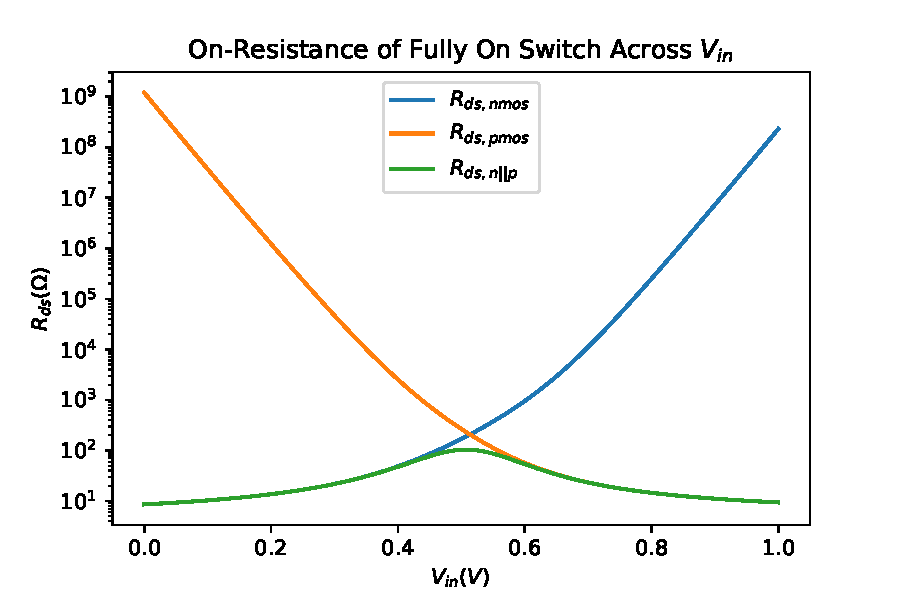
\includegraphics[width=0.8\textwidth]{figs/partb.pdf}
    \end{center}

  \item $V_{in}$'s frequency is set indirectly by the parameter \texttt{NUM\_PERIODS} which is equal to 511. Why is the frequency specified as a number of periods, and why is the value 511 (instead of e.g. 512)?

    We want to keep the number of sampled points in the transient the same so the DFT has the same noise floor across all measurements.
    Also we want an integer number of periods to avoid spectral leakage; this coherent sampling keeps all the signal power in 1 FFT bin.
    Finally \texttt{NUM\_PERIODS} is set such that GCD(\texttt{NUM\_PERIODS}, \texttt{NUM\_POINTS}) = 1 so that different sampling points are used in each cycle of the input signal.

  \item Run transient analysis for \texttt{NUM\_PERIODS} = 511, 127, 63, and 31. Plot HD3. Only use the last 16384 samples to ignore the stabilization period.

  \begin{minted}{python}
hd3 = []
for sweep in ['000', '001', '002', '003']:
    tran_sim = libpsf.PSFDataSet("problem.raw/sweep-" + sweep + "_tran.tran.tran")
    t = tran_sim.get_sweep_values()[-16384:]
    vout = tran_sim.get_signal("n2")[-16384:]
    fs = 10e6
    raw_fft = np.abs(np.fft.fft(vout))
    N = len(t)
    raw_fft = raw_fft[:int(N/2)]
    fft = 20*np.log10(2*raw_fft/N)
    f = np.array(range(0, int(N/2))) / N * fs / 1e6
    part = np.argpartition(raw_fft, -2)[-2:]
    sig_amp = raw_fft[part[0]]
    harm_amp = raw_fft[part[0]*3]
    hd3.append(harm_amp/sig_amp)
    print(harm_amp/sig_amp)
  \end{minted}

  \begin{minted}{python}
in_freq = [p/100e-9/16384 for p in [511, 127, 63, 31]]
plt.plot(in_freq, hd3)
plt.xlabel('$f_{in}$ (Hz)')
plt.ylabel('HD3')
plt.title('$f_{in}$ vs HD3')
plt.savefig('figs/partd.pdf')
  \end{minted}

  \begin{center}
    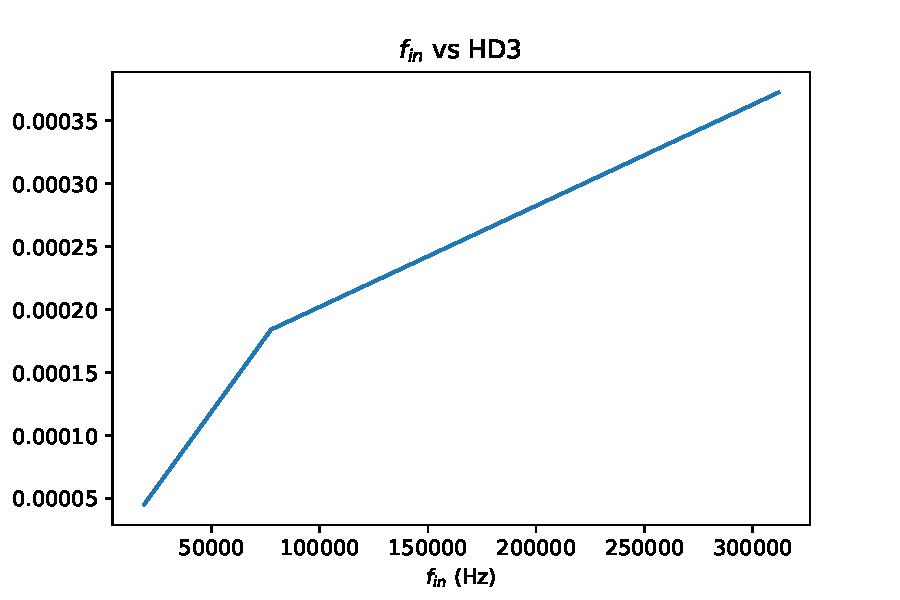
\includegraphics[width=0.8\textwidth]{figs/partd.pdf}
  \end{center}
\end{enumerate}
\end{document}
